\section{Evaluation}

\hk{Don't read this part yet, still working on it.}

The Lossy Coherence protocol was implemented and evaluated using gem5 under full-system simulation \cite{Binkert2011}. We model a tiled CMP with each tile having one core, private L1 caches, and one slice of a shared inclusive L2. Lossy Coherence extends an existing MOESI CMP directory protocol \cite{gem5_MOESI}. The simulation setup is detailed in Table. \ref{tab:machine_config}. Cache and DRAM energy is modeled using CACTI \cite{Muralimanohar2007}. We use the same benchmarks as described in the Motivation (Table. \ref{tab:benchmarks}).

\begin{table}[!t]
\caption{Simulated Machine Configuration}
	\begin{center}
		\begin{tabular}{|l|c|}
			\hline

			\textbf{Parameter} & \textbf{Values}\\
			\hline

			Cores & \makecell[l]{8 Cores, In-order, X86, 1GHz}\\
			\hline

			L1 & \makecell[l]{Private 32kB DCache/32kB ICache, \\ 2-Way Set Assoc., 64B Block, Pseudo-LRU, 2-cycle}\\
			\hline

			L2 & \makecell[l]{Shared, 128kB per core, 8-Way Set Assoc., \\ 64B Block, Pseudo-LRU, 10-cycle}\\
			\hline

			Coherence & \makecell[l]{Lossy Protocol (underlying MOESI)}\\
			\hline

			Network & \makecell[l]{2x4 Mesh, XY Routing, \\1-cycle hop router, 1-cycle hop link,\\ 4 Directory Controllers at Mesh Corners}\\
			\hline

			DRAM & \makecell[l]{2GB, DDR3 1600MHz}\\
			\hline

		\end{tabular}
	\label{tab:machine_config}
	\end{center}
\end{table}

\begin{figure}[t]
	\centerline{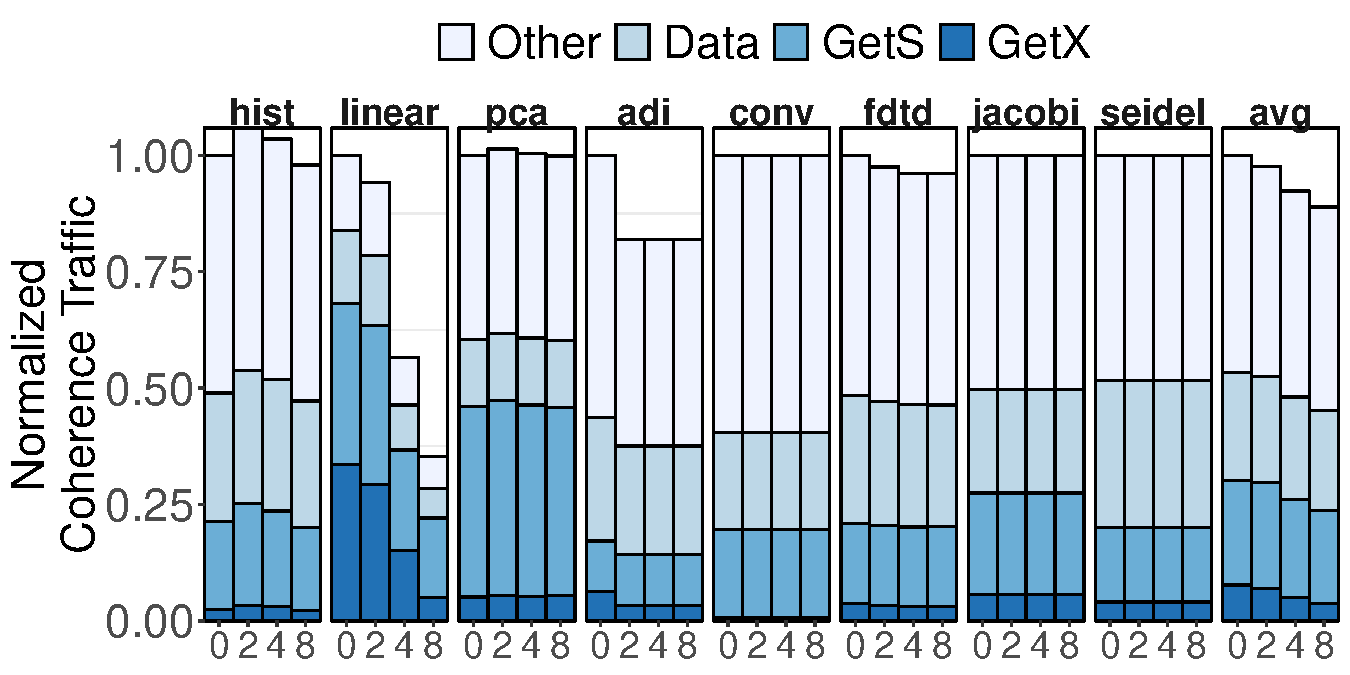
\includegraphics[scale=0.4]{graphs/coherence_saving.pdf}}
	\caption{Reduction in coherence traffic for different values of $N$ normalized to the baseline ($N = 0$) protocol. Coherence traffic is catagorized as GetX, GetS, Data, and Other.}
\label{fig:coherence_traffic}
\end{figure}

We experiment with different levels of approximation in Lossy coherence using values of $N = \{2, 4, 8\}$. Figure \ref{fig:coherence_traffic} shows a breakdown of coherence traffic where $N=0$ is the baseline protocol. We get on average 2.4\%, 7.7\%, 11.1\% reduction in coherence transactions for $N = 2, 4, 8$ respectively. Benchmark linear\_regression shows significant reduction  in coherence traffic. 64.6\%  $N = 8$, because false sharing causing high numbers of coherence misses (possible cite). L1 caches see significant reduction GetX Forwarded to remote caches from the L2 (possibly give numbers). In linear\_regression significant savings come from \storea hits on coherence invalidated line (give percentage). Similarily the adi benchmark sees a significant reduction, up to 18.0\% across all values of $N$. Benchmark adi has most \storea hits on lines in the Shared state (give percentange) which reduces GetX requests to the L2 and forwarding of data from remote caches. Coherence transaction reduction does not see much improvement for higher values of $N$ because of low temporal locality when reading and modifying data.


The reduction in coherence traffic results in energy savings within the memory heiarchy (caches and DRAM) as shown in Figure. \ref{fig:energy}. Benchmarks with greater reductions in coherence traffic correlate to greater energy savings, up to 31.5\% in $N = 8$ in linear\_regression, with 93.5\% of the energy reduction coming from the just the cache heirachy. Benchmark adi on the otherhand seeing greater savings from main memory accesses (54.4\%) of the energy savings due to silent writebacks from the L2 to Main Memory. Energy savings on average 2.4\%, 7.7\%, 11.1\% for $N = {2,4,8}$ respectively.

Figure. \ref{fig:speedup} shows the speedup gained using the Lossy Coherence compared to the baseline. Similar to energy savings, linear\_regression sees greatest speedup due to reducing the effects of false sharing, up to 67.7\% in linear\_regression and 0.8\%, 4.9\%, 9.6\% for $N = {2,4,8}$ on average across all benchmarks.

Lossy Coherence maintains an accuracy 98.4\%, 97.3\% and 96.1\% for  $N = {2,4,8}$ respectively. We measure accuracy using NRMSE.





\begin{figure}[t]
	\centerline{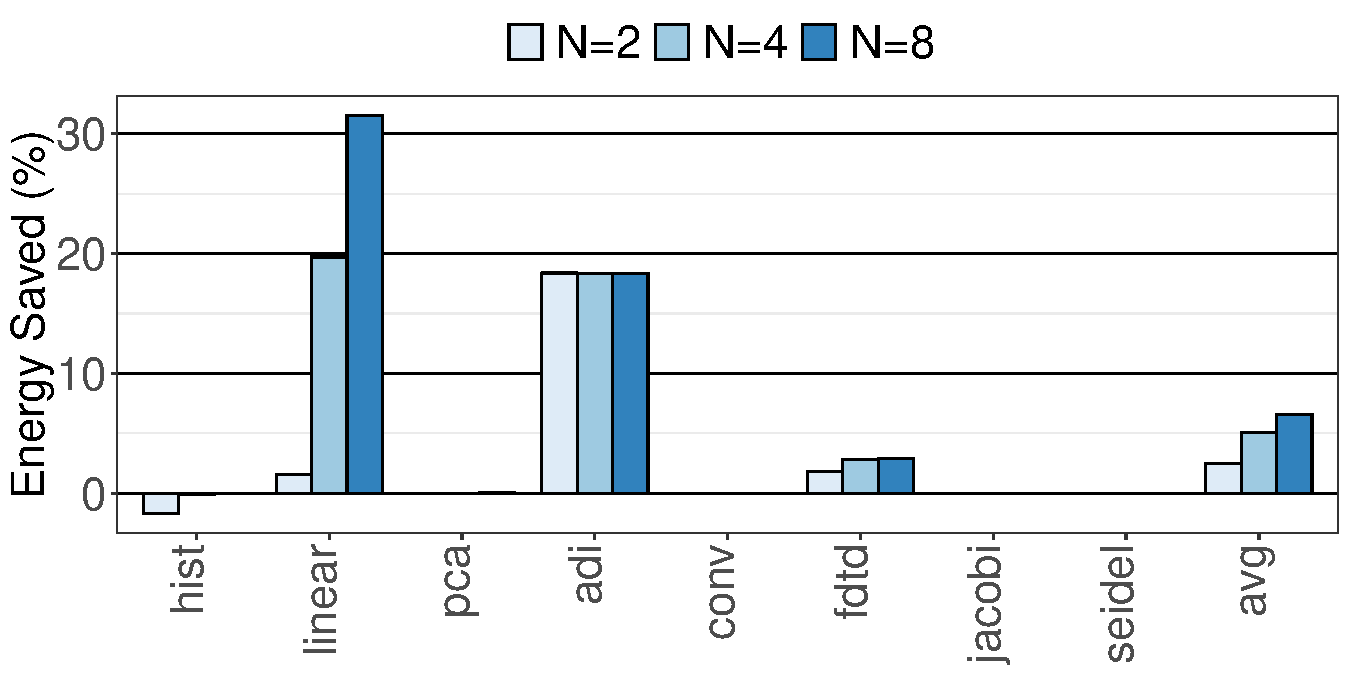
\includegraphics[scale=0.4]{graphs/energy_saved.pdf}}
	\caption{Percent energy saved within the memory heiarchy compared to the baseline for varying $N$.}
\label{fig:energy}
\end{figure}

\begin{figure}[t]
	\centerline{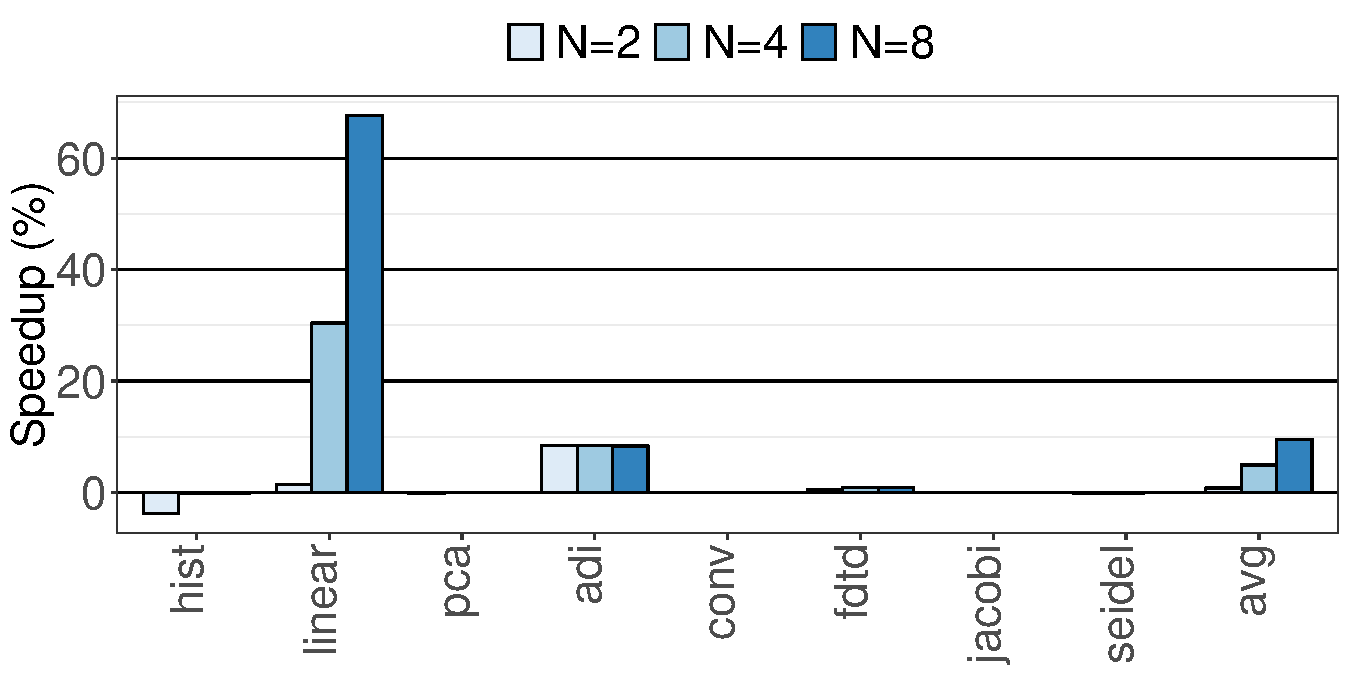
\includegraphics[scale=0.4]{graphs/speedup.pdf}}
	\caption{Percent speedup for varying $N$ compared to the baseline.}
\label{fig:speedup}
\end{figure}



\begin{figure}[t]
	\centerline{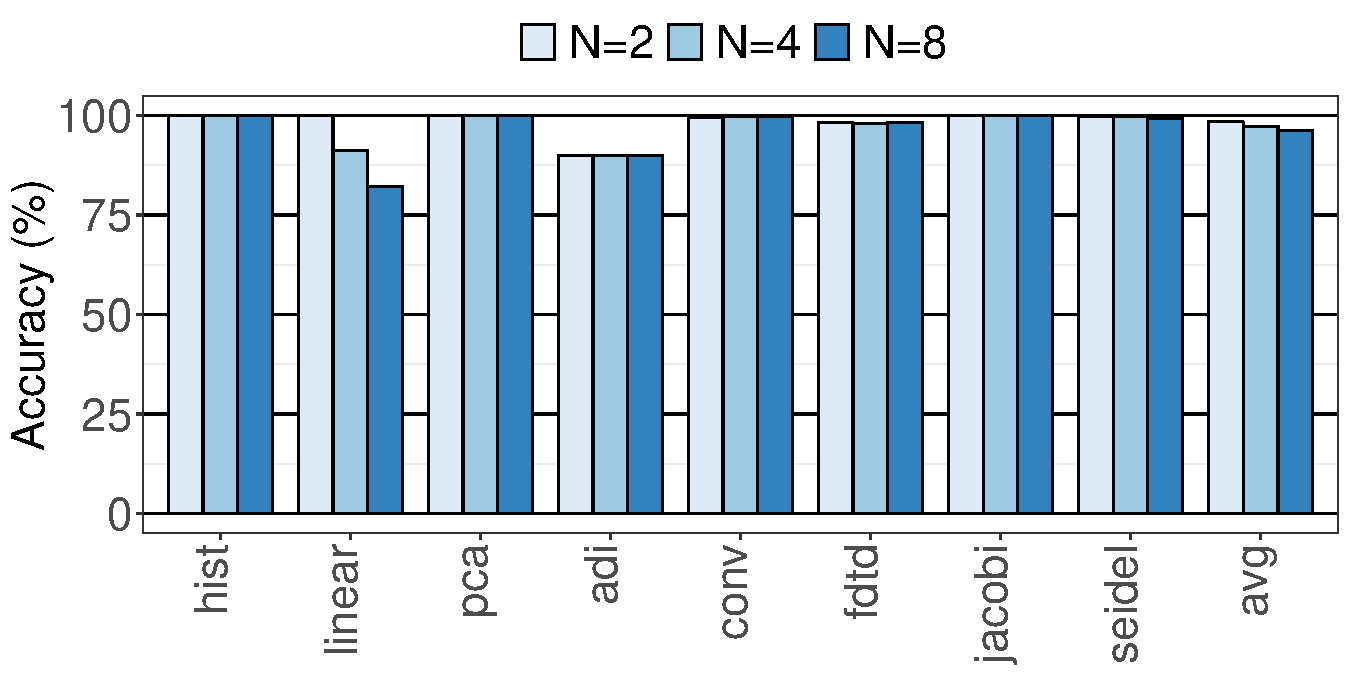
\includegraphics[scale=0.4]{graphs/output_error.pdf}}
	% \caption{TODO update plot with new orcale study data. Possible include the accuracy marker in the legend if possible.}
\label{fig:error}
\end{figure}
